\documentclass[journal]{IEEEtran}
\usepackage[utf8]{inputenc}
\usepackage[spanish]{babel}
\usepackage{enumerate}
\usepackage{graphicx}

% <------------- Librerias agregadas por Gustavo ------------------>
\usepackage{float} % para ubicar tablas en un lugar determinado [H]
\usepackage{caption}
\usepackage[caption=false]{subfig}
%\usepackage{subfigure}
\usepackage{verbatim}
\usepackage{xcolor}
\usepackage{tabularx}
\usepackage{amsmath}
\usepackage{amssymb}
\usepackage{mathtools} % para split eq
\captionsetup[figure]{name=Fig.,font=footnotesize}
\usepackage{hyperref}
\hypersetup{
    colorlinks=true,
    linkcolor=black,
    citecolor=black,      
    urlcolor=blue,
}
%\urlstyle{same}
\usepackage{lipsum}  %  dummy text para rellenar
\usepackage{enumitem}
\setlist{% configure vertical spacing for all affected lists
    font=\normalfont\itshape\color{black!80},
    %before={\color{blue!50!red}\itshape}
    }
\usepackage{subfig}
\usepackage{siunitx}
\sisetup{output-decimal-marker = {,}}
\usepackage{xfrac} % fracciones en modo texto \sfrac{1}{2}  $\sfrac{1}{2}$




\title{
    }
\author{ 
    Universidad Tecnológica Nacional 
    Facultad Regional Córdoba \\
    C\'atedra: Electrónica Aplicada III \\
    Profesor: Rivas, Guillermo \\
    Integrantes: Nicolodi, Juan Ignacio   66875 \\
    Cueva Bono, Sebastián    56016 \\
    Ruiz, Dante   49881 \\
    Albarrán, Darío Gustavo  43143 \\
    }
\date{}


% encabezado de paginas
\markboth{Electrónica Aplicada III - TP n$^\circ$2 \qquad \today}
{}


\begin{document}

\maketitle

\begin{abstract} Se diseñan dos osciladores basados en un transistor BJT MSPH10, uno de topología Clapp y otro de topología Hartley. Se simulan los circuitos en RF y se corroboran los cálculos de diseño.

\end{abstract}

\begin{IEEEkeywords}
Oscilador, Hartley, Clapp
\end{IEEEkeywords}

\section*{Introducción}
Ante el requerimiento de osciladores que trabajen en frecuencias de radio, generalmente se parte de algún diseño conocido, como son los osciladores Hartley, Colpits y Clapp \cite{randall}. En el presente informe, se pretende resolver los requerimientos de diseño de dos osciladores, basados en BJT, partiendo del las topologías Clapp y Hartley respectivamente.

El diseño de cada circuito se puede dividir en dos etapas (fig. \ref{diag01}):
\begin{itemize}
\item El amplificador propiamente dicho, que consta de un transistor NPN modelo MSPH10 \cite{MPSH10}, con su respectiva red de polarización, en modo colector común, conectado a VCC por una bobina de choque.
\item La red de realimentación, que consta de un arreglo de bobinas y capacitores, de acuerdo a la topología adoptada.
\end{itemize}

\begin{figure}[H]
\centering
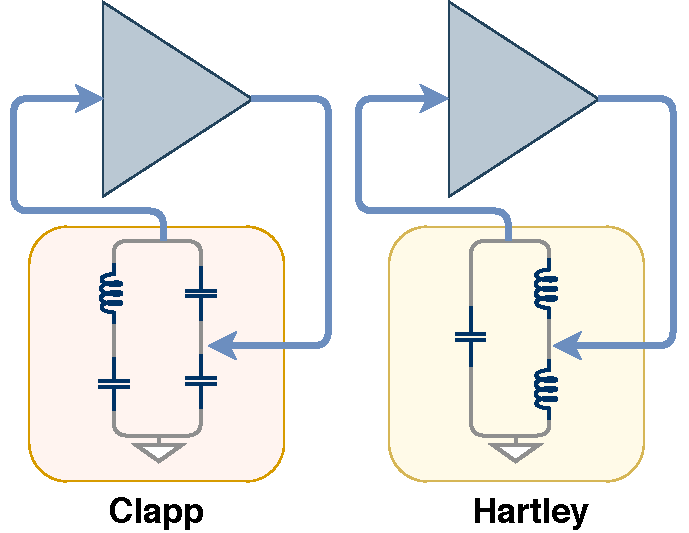
\includegraphics[width=.8\linewidth]{img/clapp_hartley-1.pdf}
\caption{Comparación entre las topologías Clapp y Hartley}
\label{diag01}
\end{figure}

También es necesario tener en cuenta, tanto para el diseño como para la simulación, la fuente de tensión y la carga, que se acopla a la malla de salida del amplificador con un capacitor.

Se realiza entonces, en primera instancia el calculo correspondiente a la polarización, para máxima excursión simétrica (M.E.S.) \cite{floyd}. Luego se calcula la red de realimentación, y finalmente se comprueba el funcionamiento en conjunto.

\section{Oscilador Clapp}
\subsection{Especificaciones:}
\begin{itemize}
    \item $f_0=\SI{100}{\mega\hertz}$
    \item $V_{CC}=\SI{12}{\volt}$
    \item $R_L=\SI{50}{\ohm}$
    \item $P_L=\SI{1}{\milli\watt}$
\end{itemize}
Transistor \emph{BJT} utilizado:
\begin{itemize}
    \item MPSH10
\end{itemize}
Según la hoja de datos:
\begin{itemize}
    \item $\beta = 60$
\end{itemize}

\subsection{Amplificador}

Amplificador clase \emph{A} en modo colector común:
\begin{align*}
    P_L &= \frac{{I_{CQ}}^2 \cdot R_L}{2}\\[1ex]
    \Rightarrow I_{CQ} &= \sqrt{\frac{2 P_L}{R_L}}\\[1ex]
    I_{CQ} &= \SI{6.3246}{\milli\ampere}\\
    \intertext{a partir de la malla de salida}
    V_{CC} &- V_{CEQ}-I_{CQ}\cdot R_E = 0\\
    \Rightarrow R_E &= \frac{V_{CC}-V_{CEQ}}{I_{CQ}}\\
    \intertext{para \emph{MES}}
    V_{CEQ} &= \frac{V_{CC}}{2}\\
    &= \SI{6}{\volt}\\
    \Rightarrow R_E &= \frac{\SI{12}{\volt} -\SI{6}{\volt}}{\SI{6.3246}{\milli\ampere}}\\
    &= \SI{948.683}{\ohm}\\
    \Aboxed{R_E &\approx \SI{1}{\kilo\ohm}}\\
    \intertext{por criterio de estabilidad}
    R_B &= \frac{\beta \cdot R_E}{10}\\
    R_B &= \SI{5.692}{\kilo\ohm}\\
    \intertext{con la ecuación de la malla de entrada}
    V_{BB} &- I_{CQ}\left( \frac{R_B}{\beta}+R_E \right) - V_{BE} = 0\\
    \Rightarrow V_{BB} &= I_{CQ}\left( \frac{R_B}{\beta}+R_E \right) + V_{BE}\\
    V_{BB} &= \SI{7.3}{\volt}\\
    R_1 &= \frac{R_B}{1-\frac{V_{BB}}{V_{CC}}}\\
    &= \SI{14.533}{\kilo\ohm}\\
    \Aboxed{R_1 &\approx \SI{15}{\kilo\ohm}}\\
    R_2 &= \frac{R_B}{\frac{V_{BB}}{V_{CC}}}\\
    &= \SI{9.357}{\kilo\ohm}\\
    \Aboxed{R_2 &\approx \SI{10}{\kilo\ohm}}
\end{align*}

%Para establecer los valores de $C_4$ y $L_2$:
Para establecer el valor del inductor de choque $L_2$:

\begin{align*}
    %X_{C_4} &\ll \frac{1}{R_L}\\
    %\Rightarrow C_4 &= \frac{R_L}{\omega}\\
    %&= \SI{79.577}{\nano\farad}\\
    %\Aboxed{C_4 &\approx \SI{80}{\nano\farad}}\\
    %\intertext{para el inductor de choque $L_2$}
    X_{L_2} &\gg Z_L\\
    \Rightarrow L_2 &= \frac{10\cdot R_L}{\omega}\\
    &= \SI{795.774}{\nano\henry}\\
    \Aboxed{L_2 &\approx \SI{800}{\nano\henry}}
\end{align*}

\begin{figure}[H]
\centering
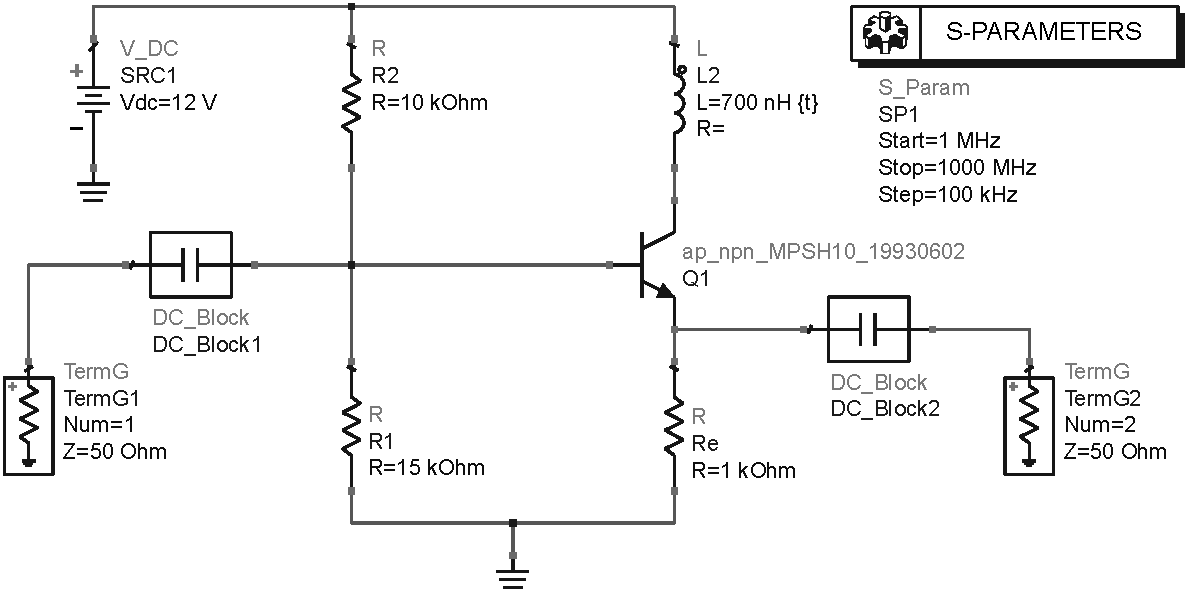
\includegraphics[width=1\linewidth]{capturas/clapp_ampli_sch-cropped.pdf}
\caption{Circuito del amplificador}
\label{fig:clapp_amp_sch}
\end{figure}
Se ajusta el inductor $L_2$ para que el amplificador trabaje en una zona mas lineal.
\begin{figure}[H]
\centering
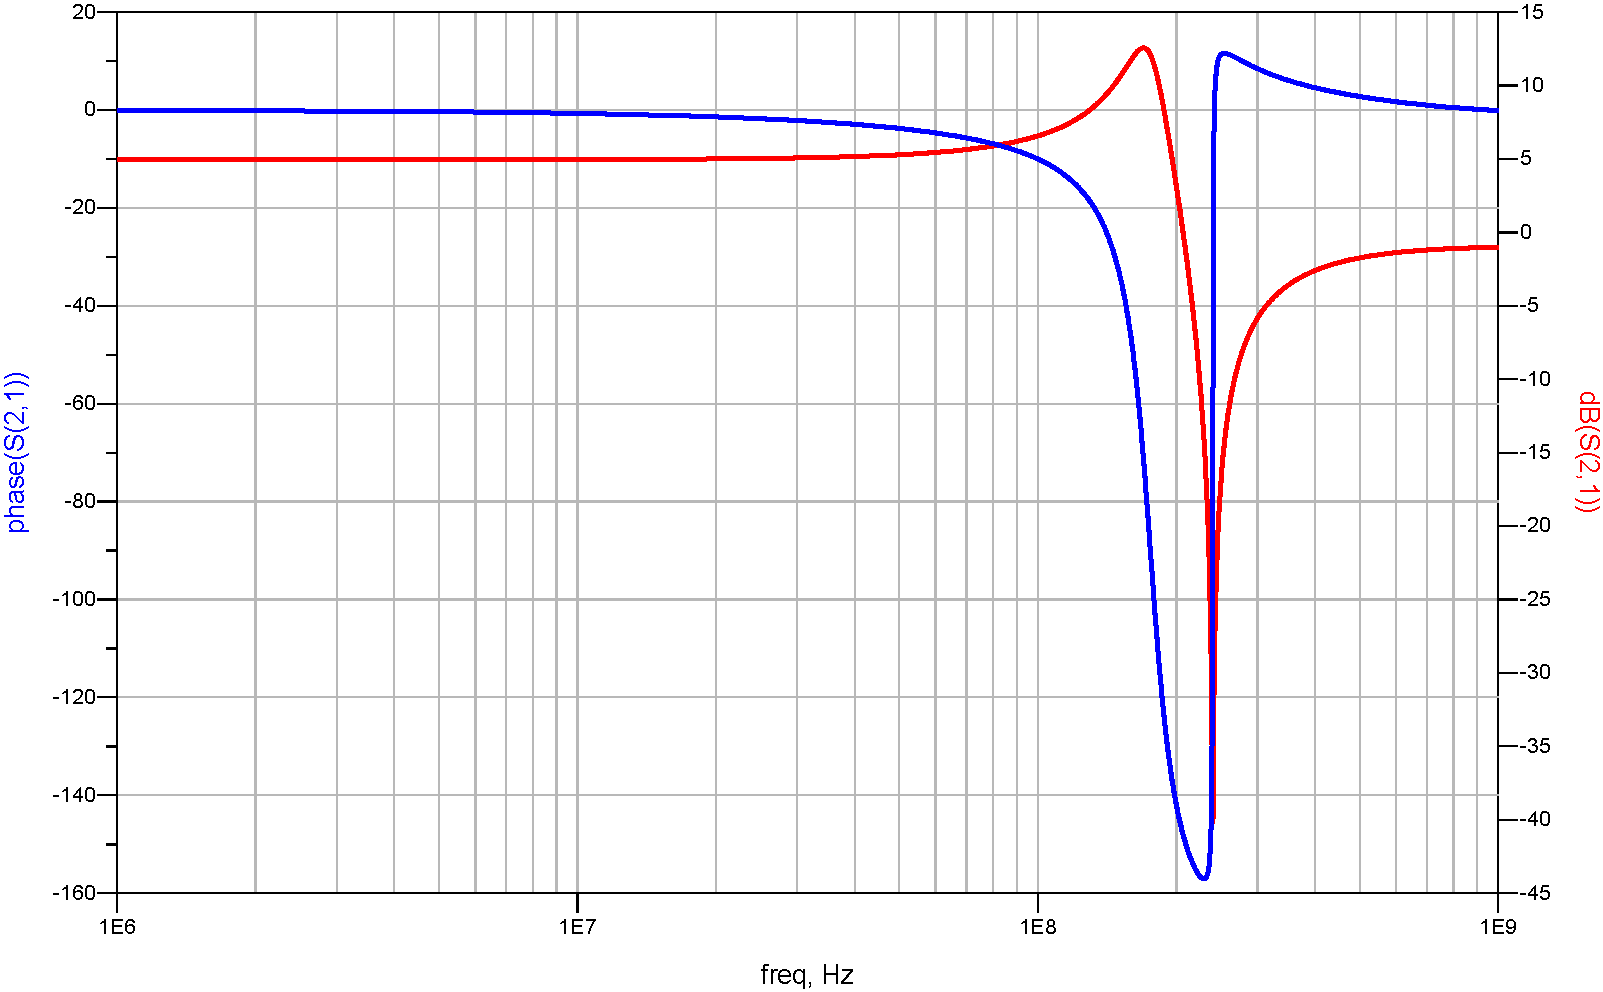
\includegraphics[width=1\linewidth]{capturas/clapp_ampli_bode-cropped.pdf}
\caption{Parámetro $S_{21}$ del amplificador}
\label{fig:clapp_amp_s21}
\end{figure}
Finalmente:
$$
    \boxed{L_2 = \SI{700}{\nano\henry}}
$$

\subsection{Resonador}
La frecuencia de resonancia del circuito de realimentación en configuración \emph{Clapp} (Fig. \ref{fig:clapp_reso_sch}):
\begin{align*}
    f_0 &=\frac{1}{2\pi \sqrt{L_1 Ct}}\\
    \intertext{donde}
    C_t &=\frac{1}{\frac{1}{C_1}+\frac{1}{C_2}+\frac{1}{C_3}}\\
    \intertext{estableciendo}
    C_2 &=C_3 \quad \text{y} \quad C_2,C_3 \gg C_1\\
    \intertext{$C_1$ domina el valor de $C_t$}
    \intertext{eligiendo}
    L_1 &=\SI{100}{\nano\henry}\\
    C_1 &= \frac{1}{(2\pi f_0)^2 L_1}\\
    &= \frac{1}{(2\pi \cdot \SI{100}{\mega\hertz})^2\cdot \SI{100}{\nano\henry}}\\
    &=\SI{25.33}{\pico\farad}\\
    \Aboxed{C_1 &\approx \SI{25}{\pico\farad}}\\
    C_2=C_3 &= 10\cdot C_1\\
    \Aboxed{C_2=C_3 &= \SI{250}{\pico\farad}}
\end{align*}
%Eligiendo  $L_1=\SI{100}{\nano\henry}$

\begin{figure}[H]
\centering
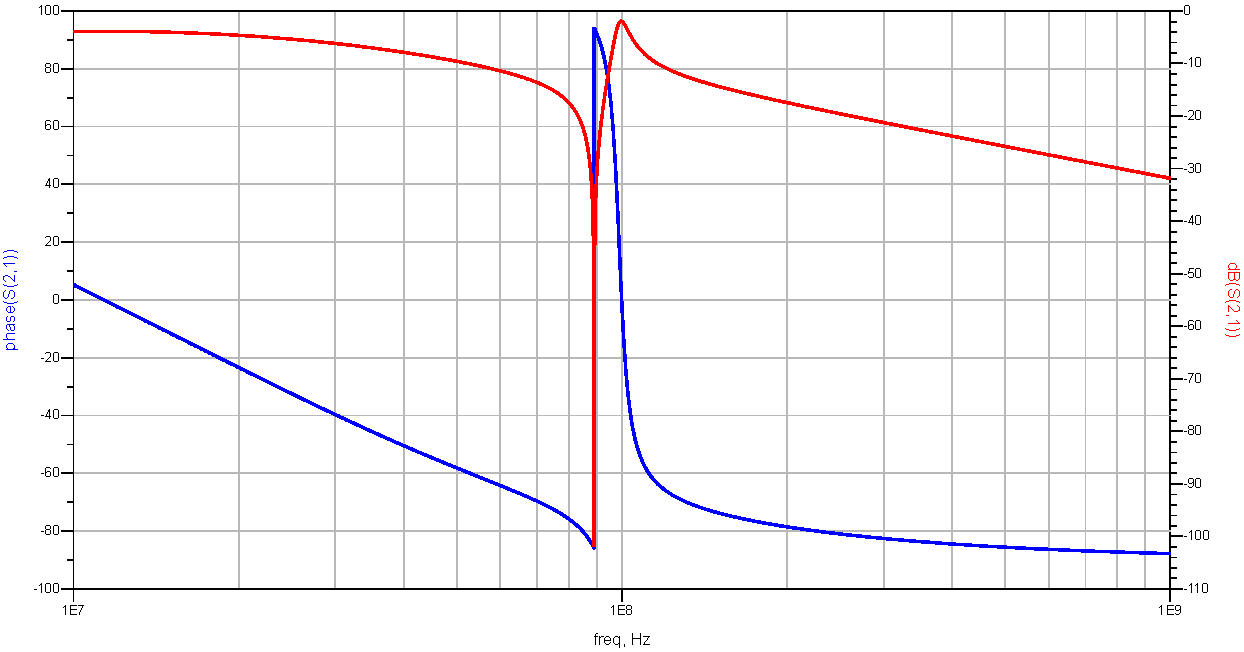
\includegraphics[width=1\linewidth]{capturas/clapp_reso_bode-cropped.pdf}
\caption{Parámetro $S_{21}$ del resonador}
\label{fig:clapp_reso_s21}
\end{figure}

Se comprueba que es necesario ajustar el capacitor $C_1$ para llevar la frecuencia de resonancia exactamente a \SI{100}{\mega\hertz}.

\begin{figure}[H]
\centering
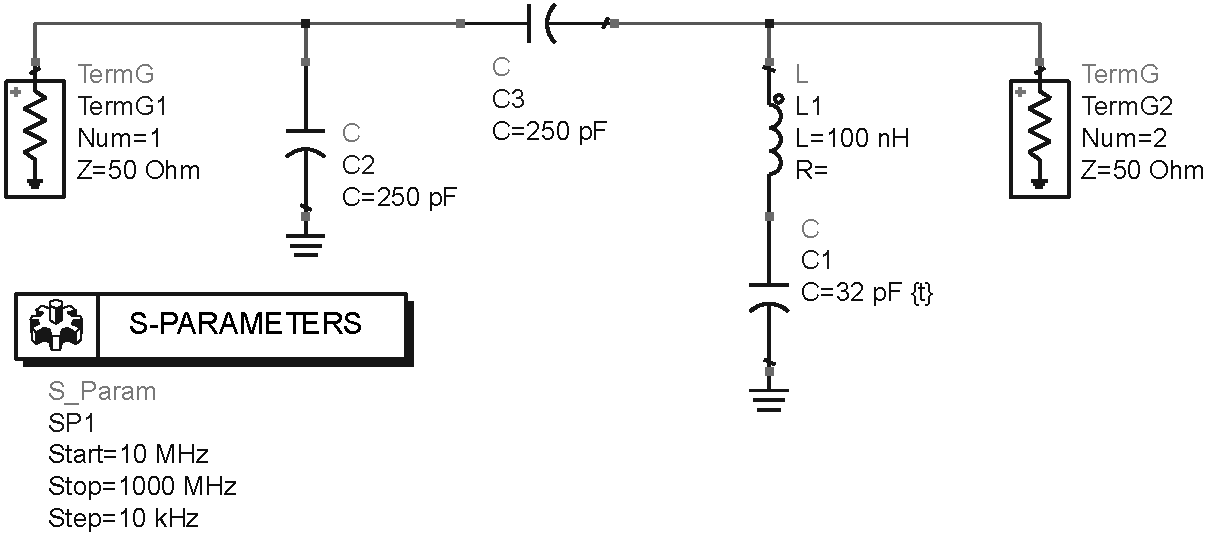
\includegraphics[width=1\linewidth]{capturas/clapp_reso_sch-cropped.pdf}
\caption{Circuito del resonador}
\label{fig:clapp_reso_sch}
\end{figure}

Finalmente:
$$
\boxed{C_1 = \SI{32}{\pico\farad}}
$$

\subsection{Oscilador}

Finalmente el oscilador queda como se ve en la figura \ref{fig:clapp_osc_sch}.

\begin{figure}[H]
\centering
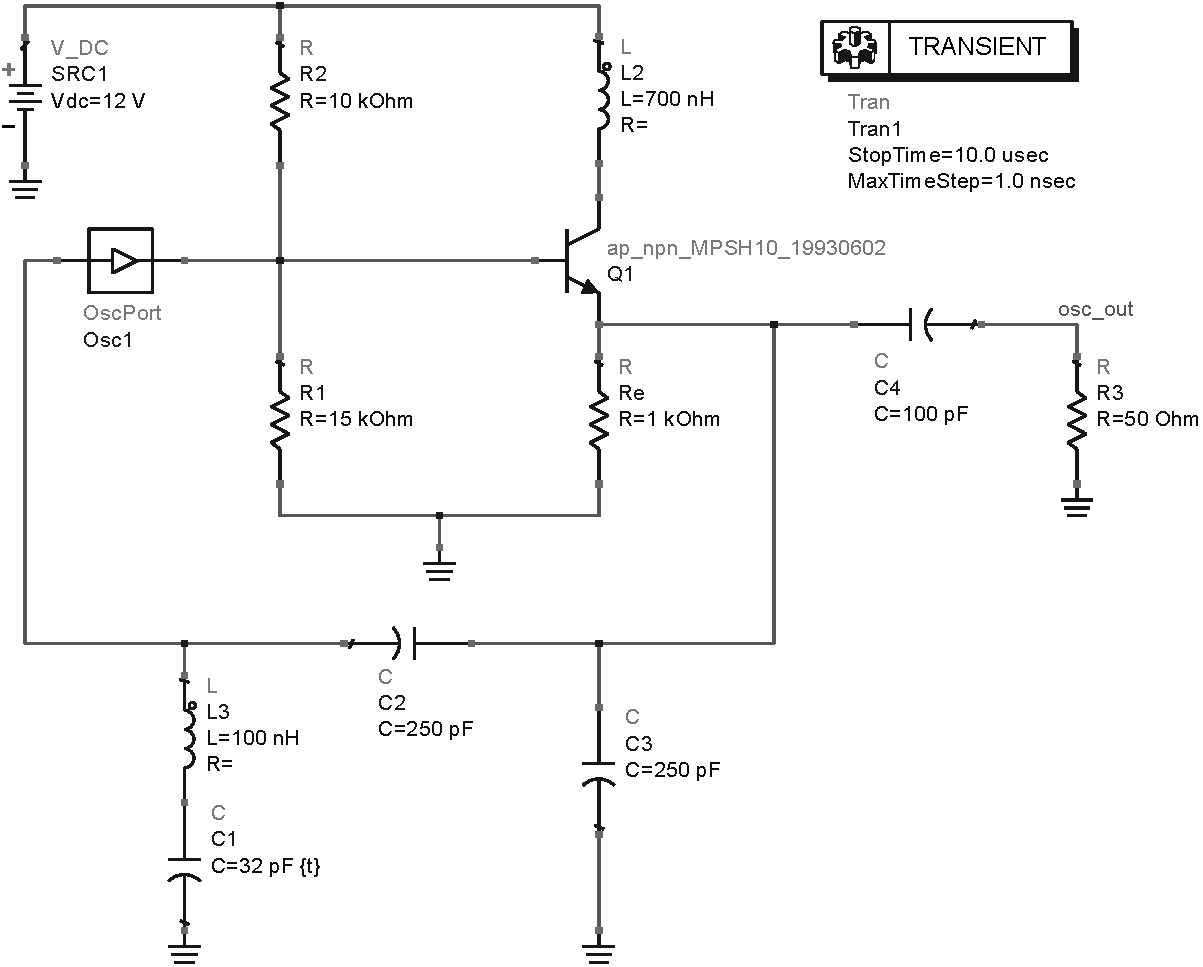
\includegraphics[width=1\linewidth]{capturas/clapp_osc_sch-cropped.pdf}
\caption{Circuito completo del oscilador Clapp}
\label{fig:clapp_osc_sch}
\end{figure}

En la figura \ref{fig:clapp_osc_trans} puede verse el proceso de arranque del oscilador.

\begin{figure}[H]
\centering
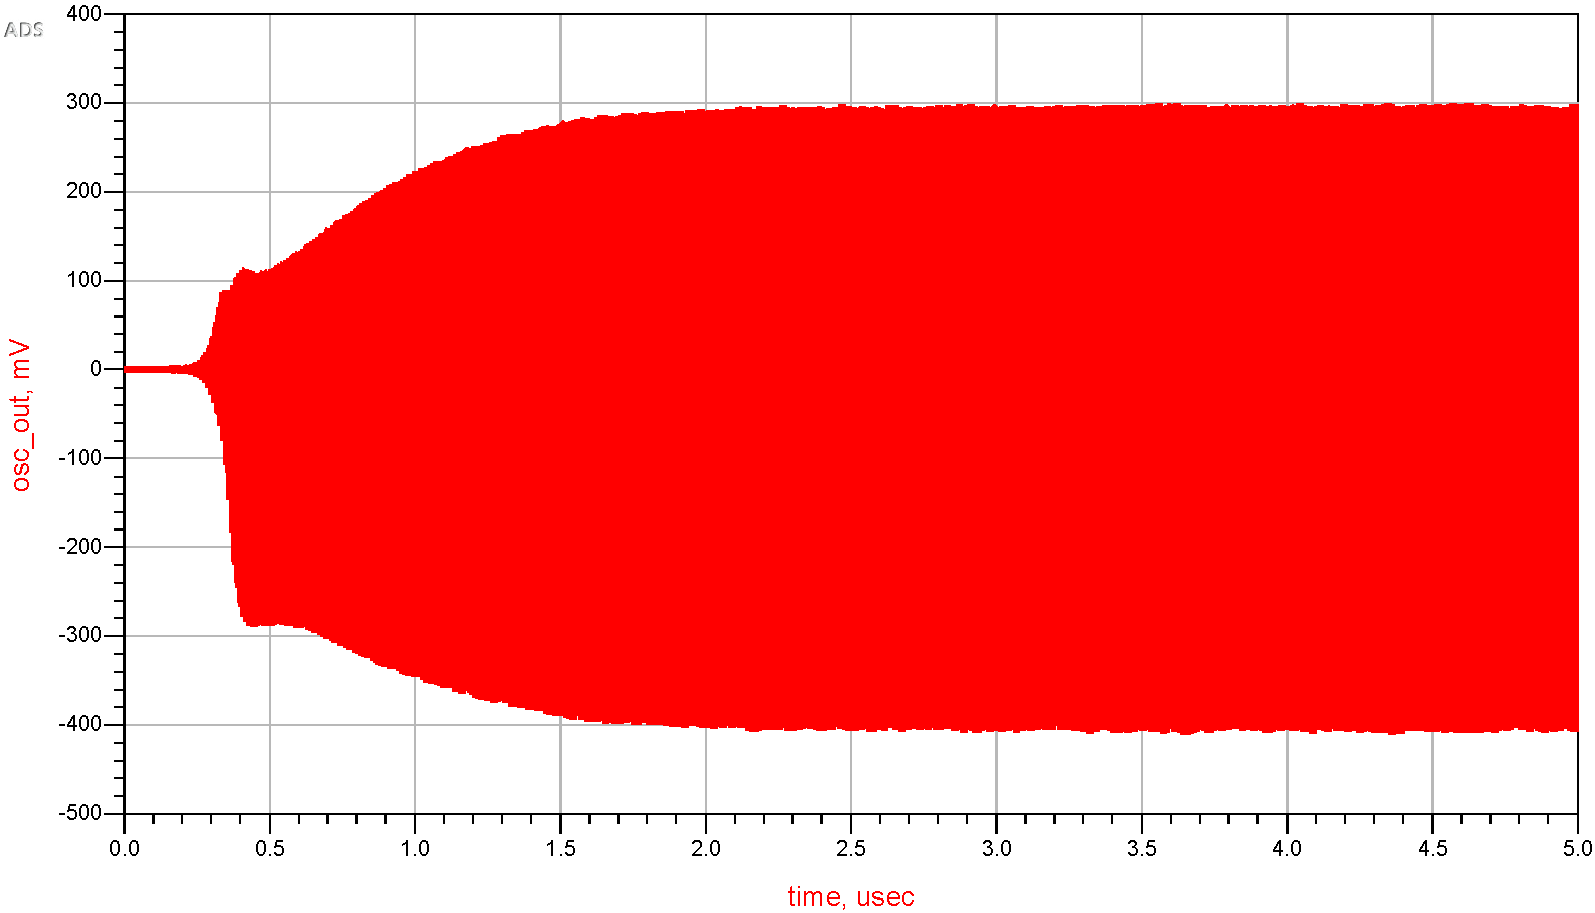
\includegraphics[width=1\linewidth]{capturas/clapp_osc_trans-cropped.pdf}
\caption{Arranque del oscilador}
\label{fig:clapp_osc_trans}
\end{figure}

Y con el oscilador en estado estacionario (Fig. \ref{fig:clapp_osc_est}) podemos medir la frecuencia de oscilación.

\begin{figure}[H]
\centering
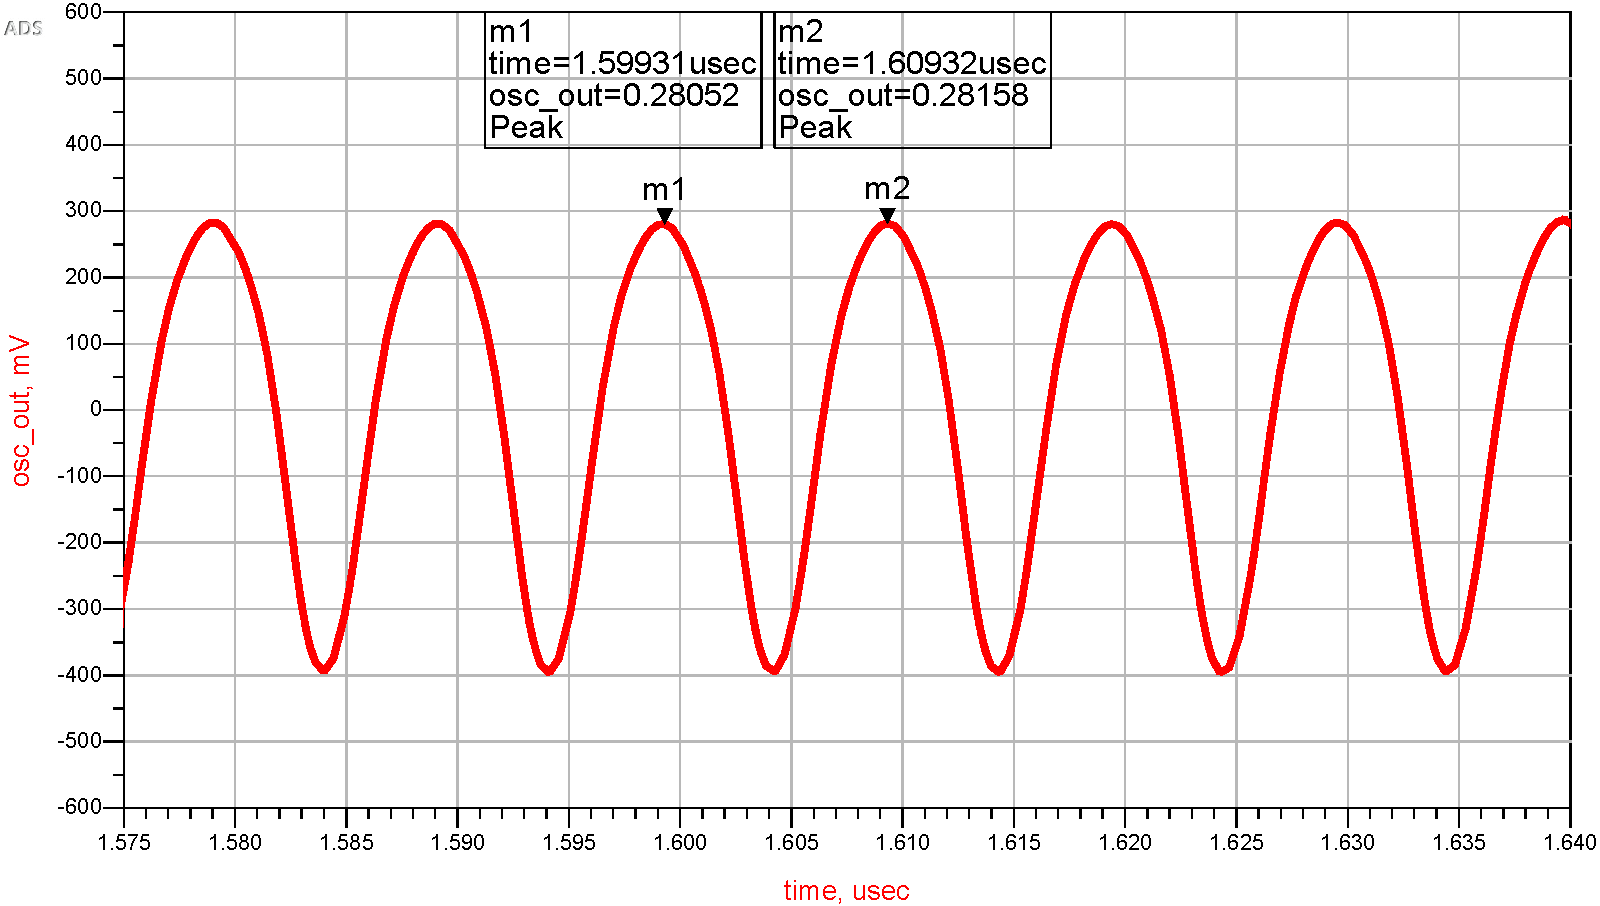
\includegraphics[width=1\linewidth]{capturas/clapp_osc_est-cropped.pdf}
\caption{oscilador en estado estacionario}
\label{fig:clapp_osc_est}
\end{figure}

Potencia disponible en la carga
$$V_L=\frac{V_p}{\sqrt{ 2 }}=212.132mV$$
$$P_L=\frac{V_L^2}{R_L}=0.9mW$$


\section{Oscilador Hartley}
\subsection{Especificaciones:}
\begin{itemize}
    \item $f_0=\SI{10}{\mega\hertz}$
    \item $V_{CC}=\SI{12}{\volt}$
    \item $R_L=\SI{50}{\ohm}$
    \item $P_L=\SI{5}{\milli\watt}$
\end{itemize}
Transistor \emph{BJT} utilizado:
\begin{itemize}
    \item MPSH10
\end{itemize}
Según la hoja de datos:
\begin{itemize}
    \item $\beta = 60$
\end{itemize}

\subsection{Amplificador}
Se utiliza un amplificador con la misma topologia empleada en el oscilador  \emph{Clapp} modificando la inductancia de L2 y la polarización según los requerimientos de potencia.
\begin{align*}
    P_L &= \frac{{I_{CQ}}^2 \cdot R_L}{2}\\[1ex]
    \Rightarrow I_{CQ} &= \sqrt{\frac{2 P_L}{R_L}}\\[1ex]
    I_{CQ} &= \SI{14.14}{\milli\ampere}\\
    \intertext{a partir de la malla de salida}
    V_{CC} &- V_{CEQ}-I_{CQ}\cdot R_E = 0\\
    \Rightarrow R_E &= \frac{V_{CC}-V_{CEQ}}{I_{CQ}}\\
    \intertext{para \emph{MES}}
    V_{CEQ} &= \frac{V_{CC}}{2}\\
    &= \SI{6}{\volt}\\
    \Rightarrow R_E &= \frac{\SI{12}{\volt} -\SI{6}{\volt}}{\SI{14.14}{\milli\ampere}}\\
    &= \SI{424.264}{\ohm}\\
    \Aboxed{R_E &\approx \SI{470}{\ohm}}\\
    \intertext{por criterio de estabilidad}
    R_B &= \frac{\beta \cdot R_E}{10}\\
    R_B &= \SI{2.5456}{\kilo\ohm}\\
    \intertext{con la ecuación de la malla de entrada}
    V_{BB} &- I_{CQ}\left( \frac{R_B}{\beta}+R_E \right) - V_{BE} = 0\\
    \Rightarrow V_{BB} &= I_{CQ}\left( \frac{R_B}{\beta}+R_E \right) + V_{BE}\\
    V_{BB} &= \SI{7.3}{\volt}\\
    R_1 &= \frac{R_B}{1-\frac{V_{BB}}{V_{CC}}}\\
    &= \SI{6.4994}{\kilo\ohm}\\
    \Aboxed{R_1 &\approx \SI{6.5}{\kilo\ohm}}\\
    R_2 &= \frac{R_B}{\frac{V_{BB}}{V_{CC}}}\\
    &= \SI{4.1845}{\kilo\ohm}\\
    \Aboxed{R_2 &\approx \SI{4.5}{\kilo\ohm}}
\end{align*}

%Para establecer los valores de $C_4$ y $L_2$:
Para establecer el valor del inductor de choque $L_2$:
\begin{align*}
    %X_{C_4} &\ll \frac{1}{R_L}\\
    %\Rightarrow C_4 &= \frac{R_L}{\omega}\\
    %&= \SI{79.577}{\nano\farad}\\
    %\Aboxed{C_4 &\approx \SI{80}{\nano\farad}}\\
    %\intertext{para el inductor de choque $L_2$}
    X_{L_2} &\gg Z_L\\
    \Rightarrow L_2 &= \frac{10\cdot R_L}{\omega}\\
    &= \SI{7.957}{\micro\henry}\\
    \Aboxed{L_2 &\approx \SI{8}{\micro\henry}}
\end{align*}

\begin{figure}[H]
\centering
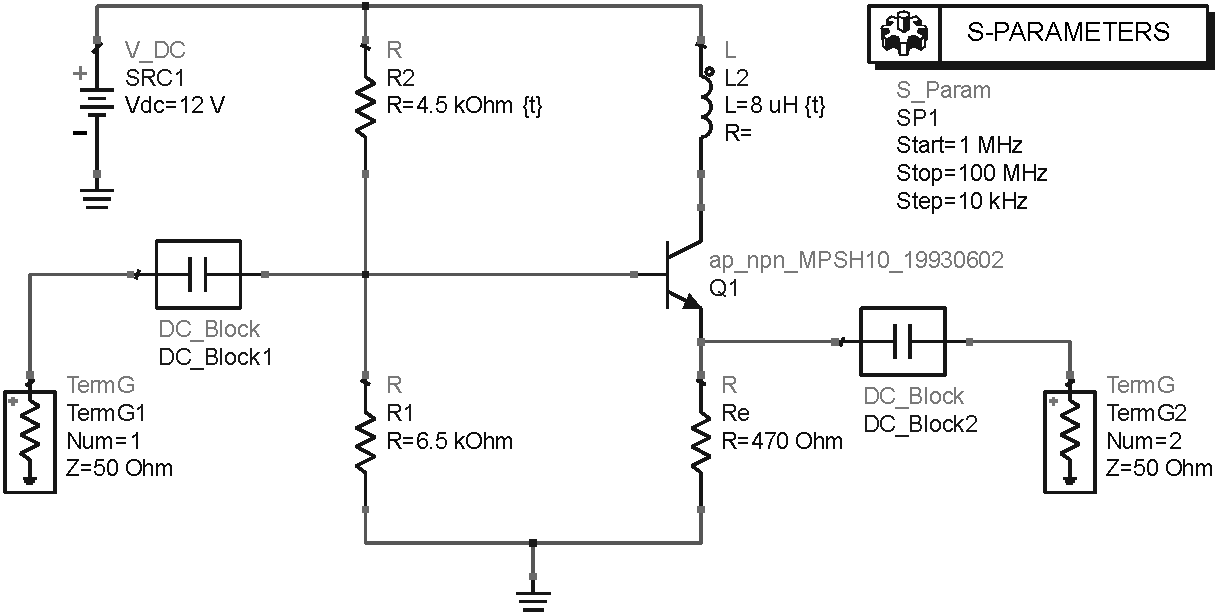
\includegraphics[width=1\linewidth]{capturas/hartley_ampli_sch-cropped.pdf}
\caption{Circuito del amplificador}
\label{fig:hartley_amp_sch}
\end{figure}

\begin{figure}[H]
\centering
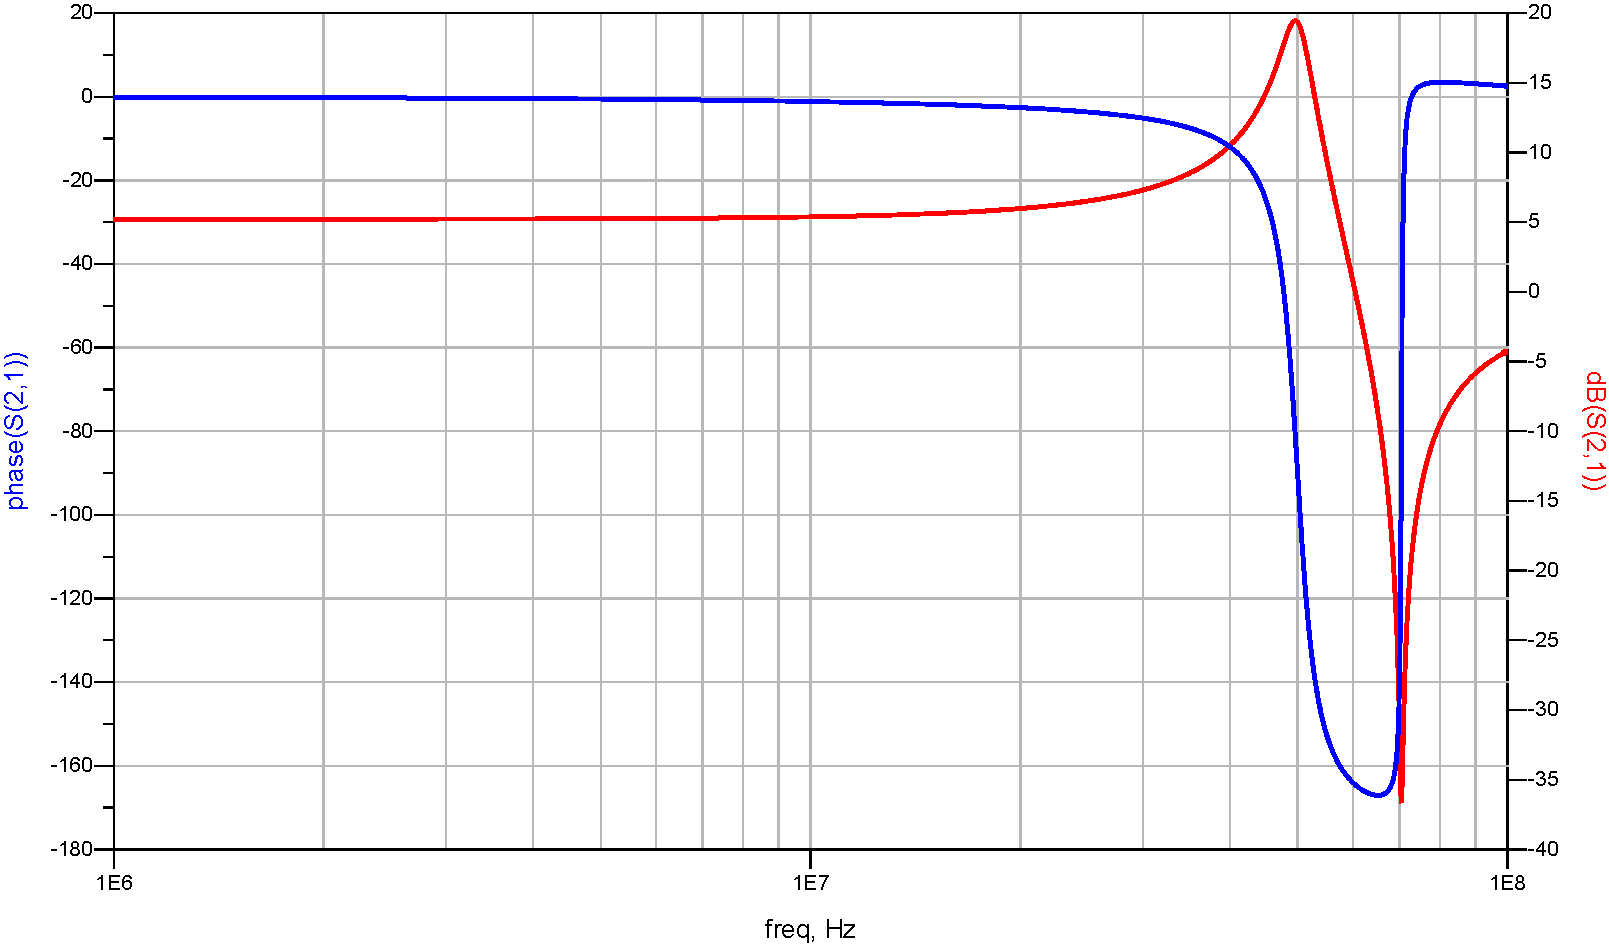
\includegraphics[width=1\linewidth]{capturas/hartley_ampli_bode-cropped.pdf}
\caption{Parámetro $S_{21}$ del amplificador}
\label{fig:hartley_amp_s21}
\end{figure}

Se comprueba que el amplificador trabaja en una zona lineal para la frecuencia de oscilación.


\subsection{Resonador}
La frecuencia de resonancia de la malla de realimentación en configuración \emph{Hartley} (Fig. \ref{fig:hartley_reso_sch}):
\begin{align*}
    f_0 &=\frac{1}{2\pi \sqrt{L_1 C_1}}\\
    \intertext{donde}
    L_1  &= L_{1a} + L_{1b}\\
    L_{1b} &= 10 \times L_{1a}\\
    \intertext{eligiendo}
    L_1     &\approx \SI{100}{\nano\henry}\\
    L_{1b}  &=\SI{90}{\nano\henry}\\
    L_{1a}  &=\SI{9}{\nano\henry}\\
    C_1 &= \frac{1}{(2\pi f_0)^2 L_1}\\
    &= \frac{1}{(2\pi \cdot \SI{10}{\mega\hertz})^2\cdot \SI{100}{\nano\henry}}\\
    &=\SI{2.533}{\nano\farad}\\
    \Aboxed{C_1 &\approx \SI{2.5}{\nano\farad}}
\end{align*}

\begin{figure}[H]
\centering
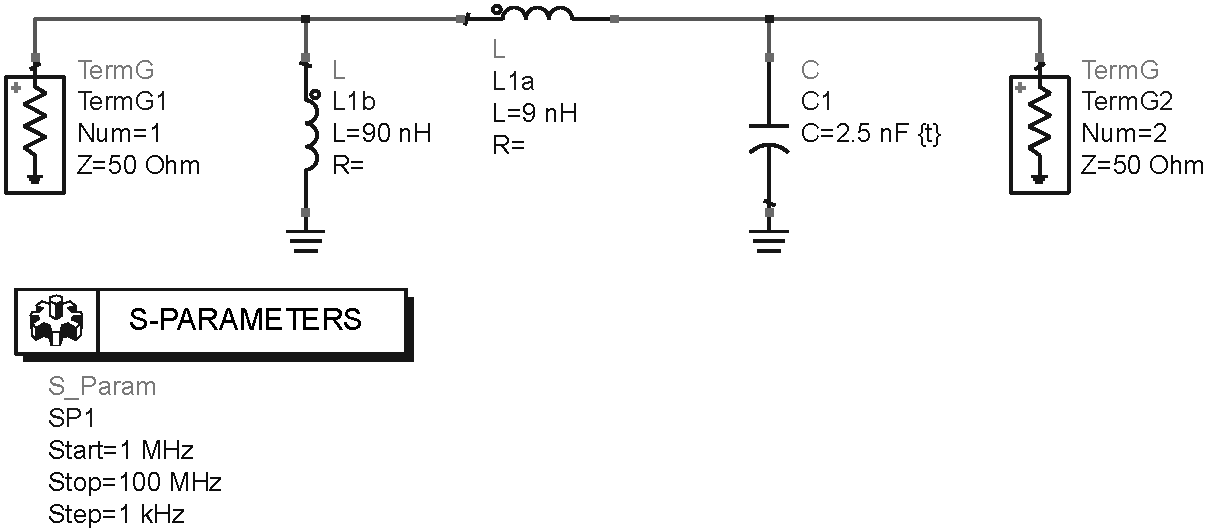
\includegraphics[width=1\linewidth]{capturas/hartley_reso_sch-cropped.pdf}
\caption{Circuito del resonador}
\label{fig:hartley_reso_sch}
\end{figure}

\begin{figure}[H]
\centering
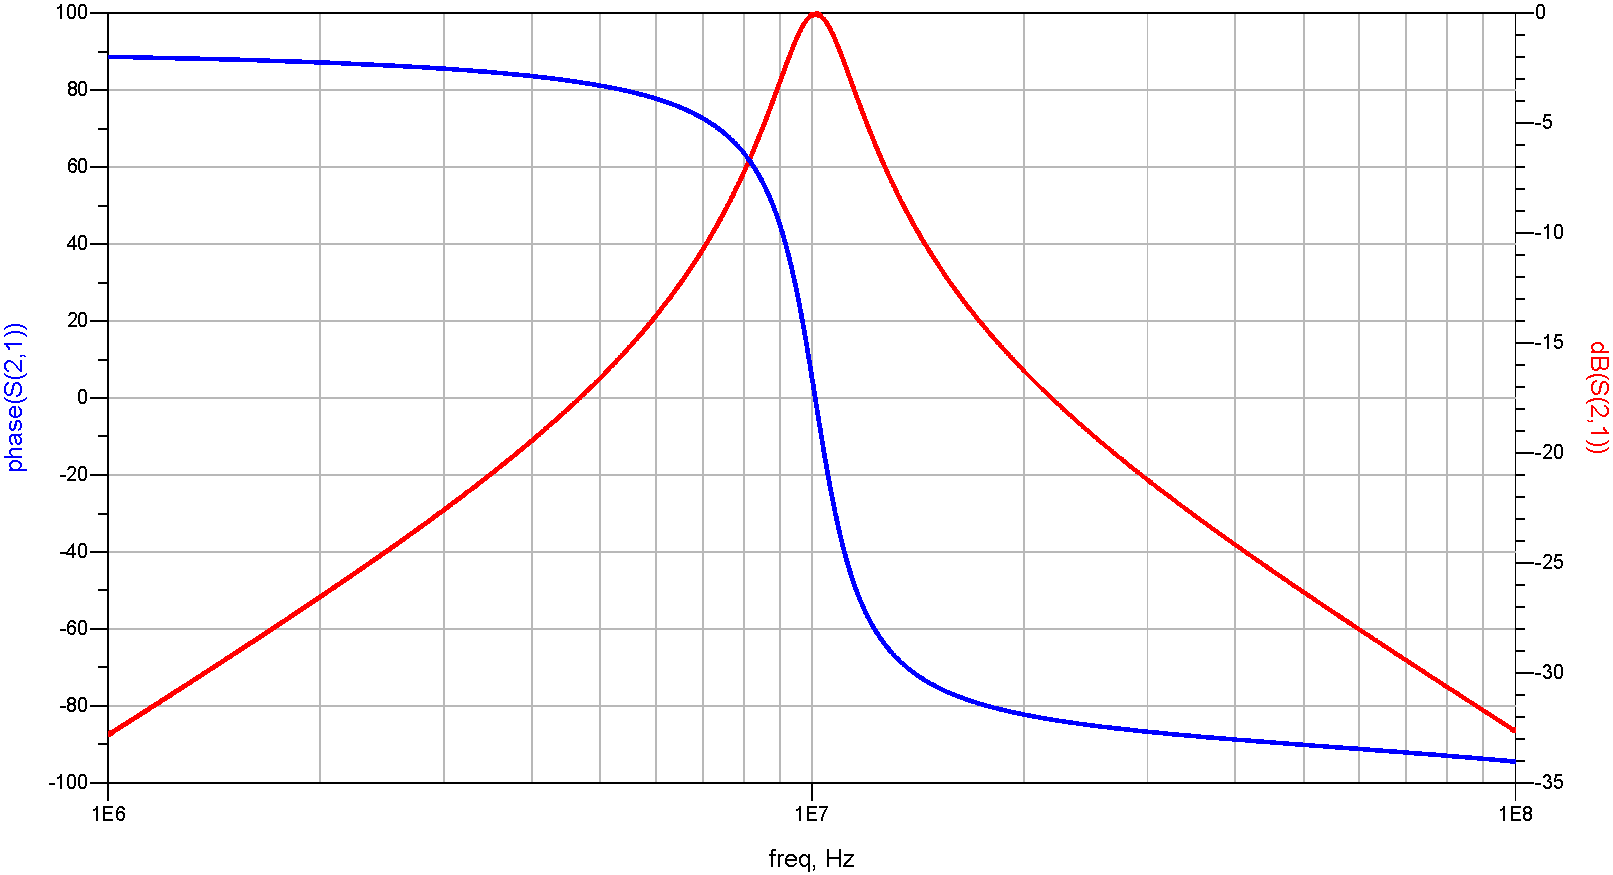
\includegraphics[width=1\linewidth]{capturas/hartley_reso_bode-cropped.pdf}
\caption{Parámetro $S_{21}$ del resonador}
\label{fig:hartley_reso_s21}
\end{figure}

El circuito resuena exactamente a la frecuencia de diseño.

\subsection{Oscilador}

El oscilador completo puede verse en la figura \ref{fig:hartley_osc_sch}.

\begin{figure}[H]
\centering
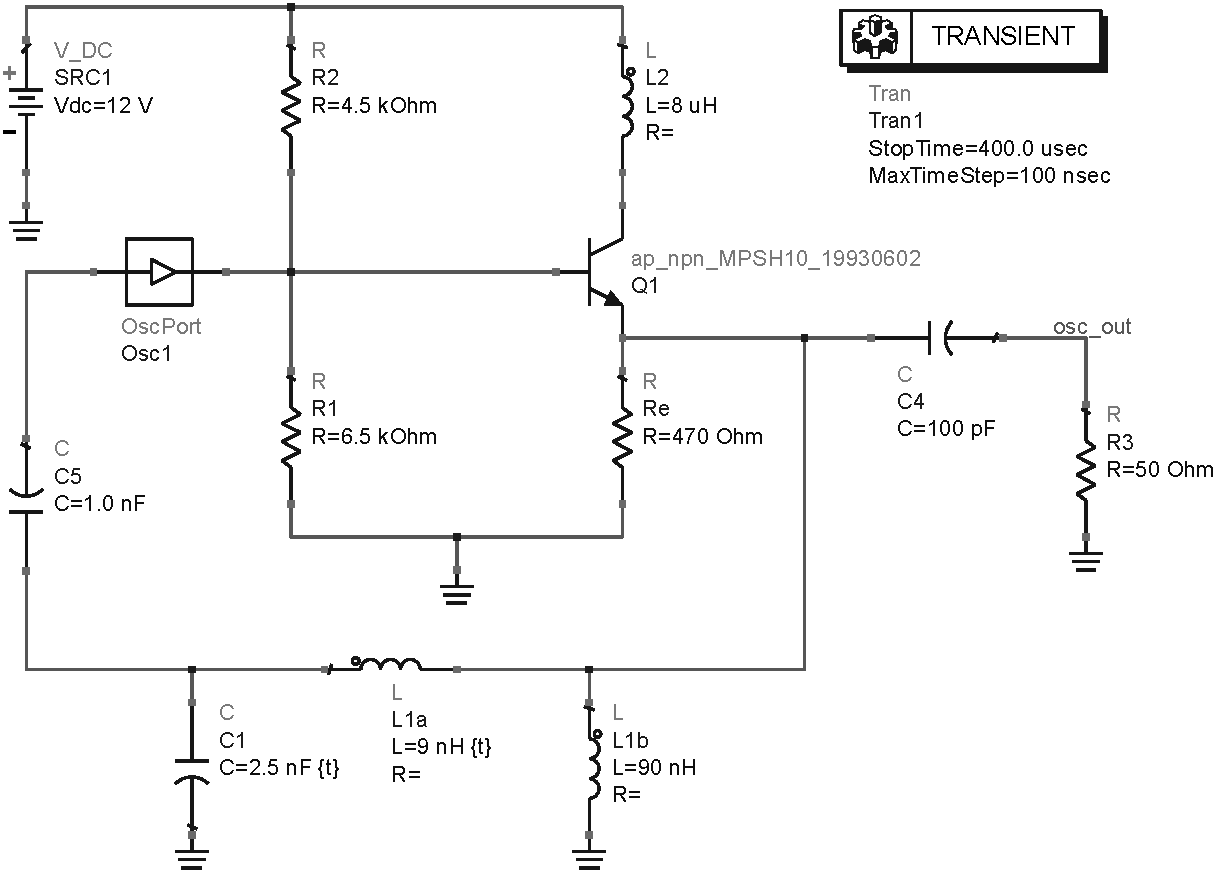
\includegraphics[width=1\linewidth]{capturas/hartley_osc_sch-cropped.pdf}
\caption{Circuito completo del oscilador Hartley}
\label{fig:hartley_osc_sch}
\end{figure}

El proceso de arranque del oscilador Hartley es mucho mas lento que el Clapp, como puede verse en la figura \ref{fig:hartley_osc_trans}.

\begin{figure}[H]
\centering
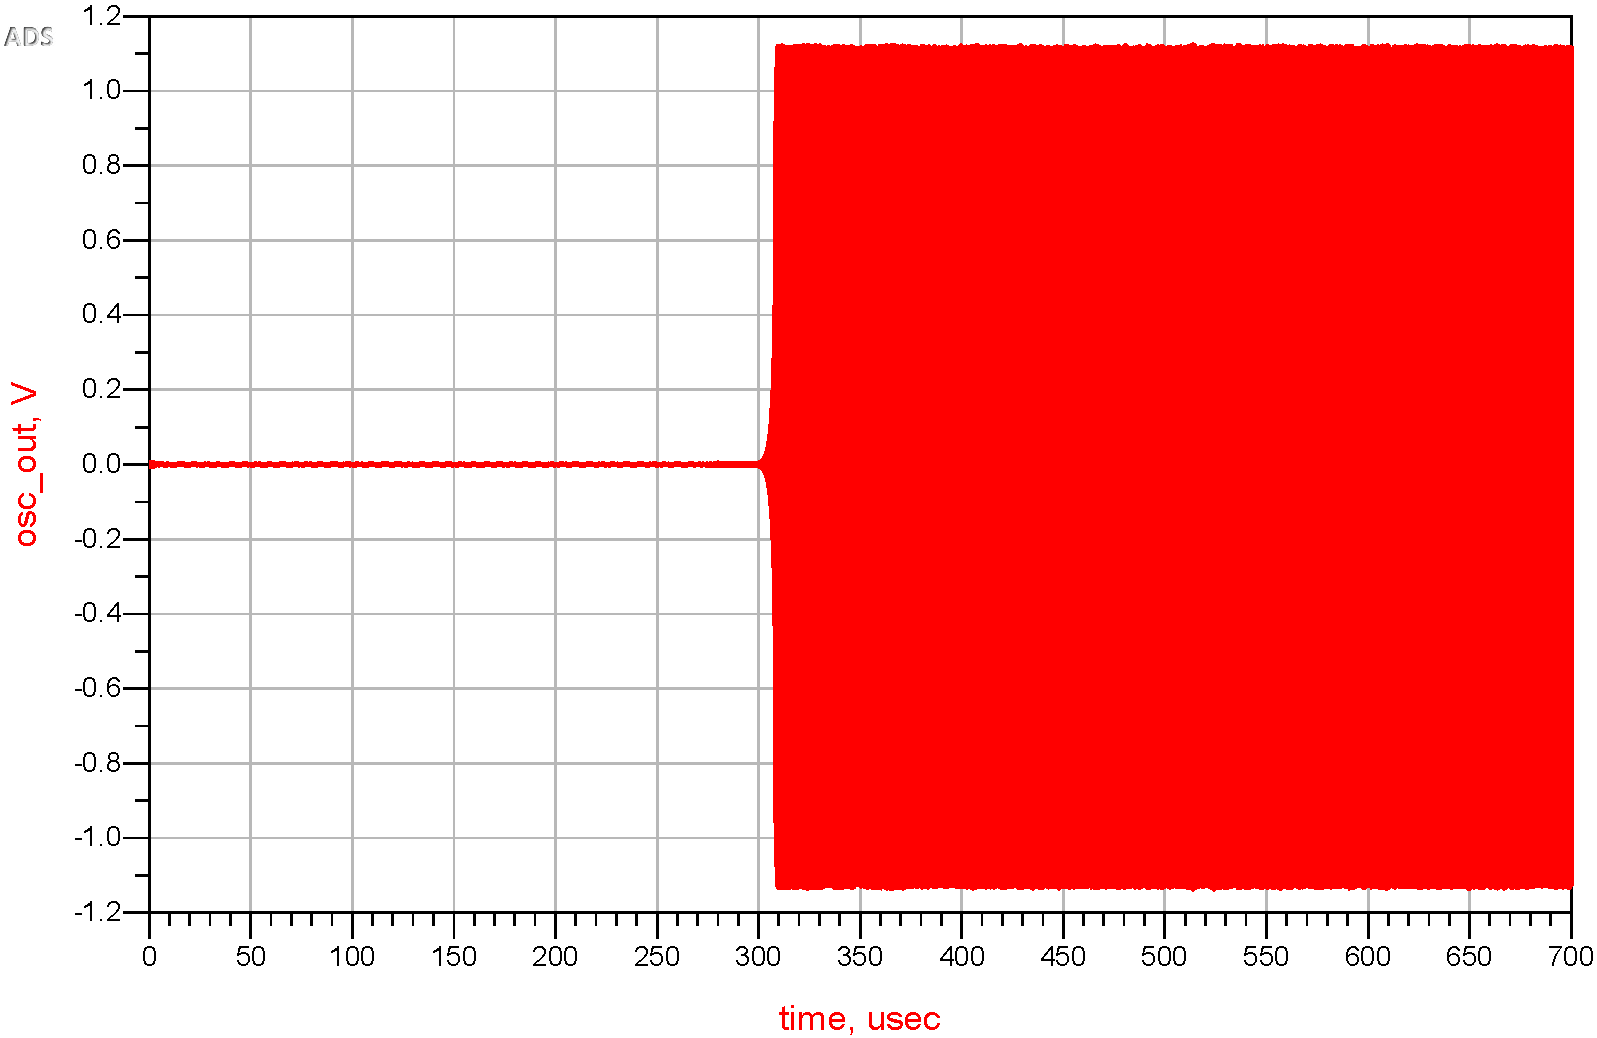
\includegraphics[width=1\linewidth]{capturas/hartley_osc_trans-cropped.pdf}
\caption{Arranque del oscilador}
\label{fig:hartley_osc_trans}
\end{figure}

Con el oscilador en estado estacionario (Fig. \ref{fig:hartley_osc_est}) podemos comprobar la frecuencia de oscilación.

\begin{figure}[H]
\centering
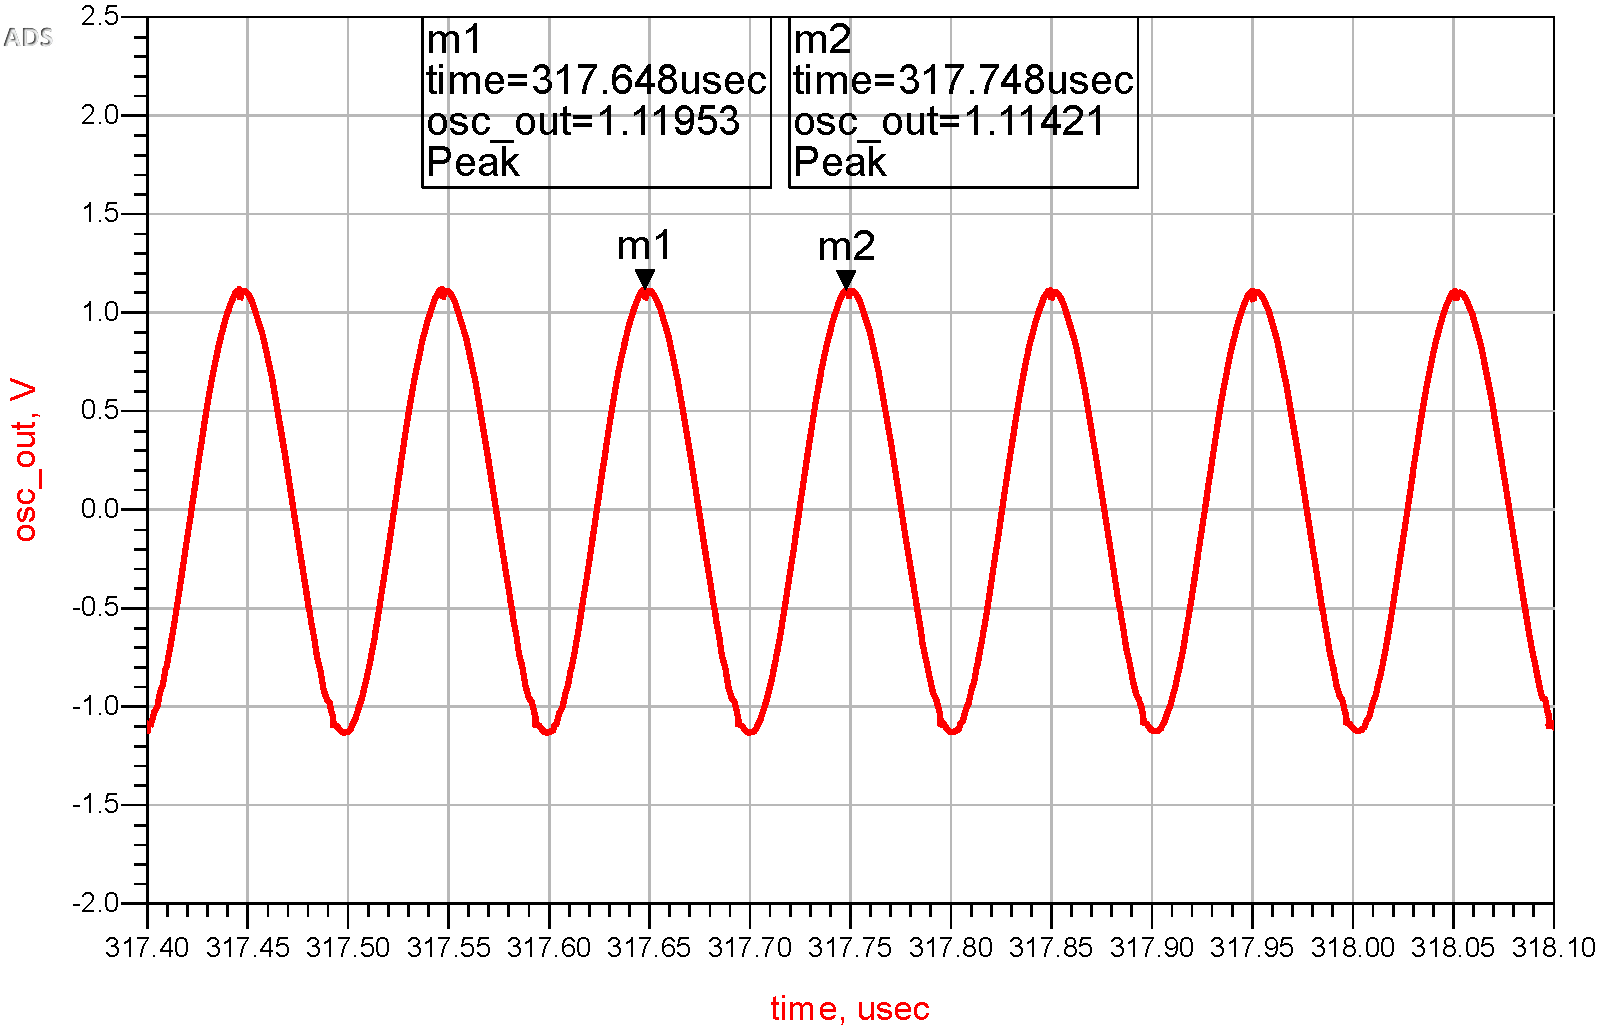
\includegraphics[width=1\linewidth]{capturas/hartley_osc_est-cropped.pdf}
\caption{oscilador en estado estacionario}
\label{fig:hartley_osc_est}
\end{figure}

Potencia disponible en la carga:

$$V_L=\frac{V_p}{\sqrt{ 2 }}=0.788mV$$
$$P_L=\frac{V_L^2}{R_L}=12.42mW$$

\section{Conclusiones}
Las dos topologías utilizadas permitieron obtener diseños que se ajusten a diferentes requerimientos.
Partiendo de los modelos básicos, y mediante los criterios de diseño, se calcularon valores para los componentes que permitieron poner en funcionamiento los osciladores. 

En el caso del oscilador \emph{Hartley}, la simulación arrojó un resultado idéntico al esperado, e incluso se obtuvo una potencia de salida simulada mayor a la requerida.

Por otra parte, en el caso del oscilador \emph{Clapp}, se debieron realizar ajustes en L2 y C1 para lograr cumplir con los requerimientos. Ajustando el valor de L2 se logró desplazar el punto de trabajo a una zona mas lineal, logrando una ganancia mayor a 0dB y con fase cercana a cero grados. Esto es necesario para obtener una oscilación estable y con baja distorsión.



\begin{thebibliography}{00}
% Agreguen la referencia a la bibliografía en el texto con  ->  \cite{autor}
\bibitem{randall} Randall W. Rhea. Discrete Oscillator Design
\bibitem{kyung} Kyung-Whan Yeom. Microwave Circuit Design: A Practical Approach Using ADS. 2015. 
\bibitem{MPSH10} MPSH10 Datasheet. Fairchild Semiconductor. 
\bibitem{floyd} Dispositivos Electrónicos, Thomas Floyd, 8va edición.
\end{thebibliography}


\end{document}
